\section{Method}
\label{sec:method}

% Enough detail to reimplement; hyperparameters are in Section~\ref{sec:setup}.
% Use one term per concept throughout: real-only, data budget, generated images, generated set.

\subsection{Data and budgets}
% Moved from the report's protocol paragraph.
The study uses CIFAR-100~\cite{krizhevsky2009learning}. The split is fixed by a manifest with seed 42: 50 images per class (5,000 in total) are held out from the training pool for validation, and the 5, 10, 20 and 50 images-per-class budgets are nested subsets of the remaining 45,000 images, which form the full budget. The official 10,000-image test set is scored once per run, after the training and selection protocol was fixed.

\subsection{Classifiers}
% Moved from the report.
ResNet-50~\cite{he2016deep} and ViT-B/16~\cite{dosovitskiy2021image} are trained with all layers updated, either from ImageNet weights (torchvision \texttt{IMAGENET1K\_V2} and \texttt{IMAGENET1K\_V1}) or from random initialization. Images stay at $32\times32$ until they are upsampled to $224\times224$ on the GPU and normalized with the ImageNet statistics.
% TODO: ConvNeXt-T (Stage 2 check of the sign flip), with a verified reference.

\subsection{Training conditions}
% Moved from the report.
Each condition is defined as one change to the real-only control. \textit{Real-only} trains on the real images of the budget without augmentation. \textit{RandAugment}~\cite{cubuk2020randaugment} applies two RandAugment operations at magnitude 9 to every training image. \textit{Pretrained Stable Diffusion} adds generated images to the real-only training set, one generated image per real image (synthetic:real 1:1): for a budget of $k$ images per class, the first $k$ generated images of each class are added, so the generated sets are nested across budgets in the same way as the real ones. \textit{Pretrained Stable Diffusion with RandAugment} uses the same pool and applies RandAugment to every image, so that a gain from generated images can be separated from the gain of augmentation in general. \textit{LoRA-adapted Stable Diffusion} replaces the pool with images from an adapter fitted only on the real images of the same budget, so each budget has its own generated set.

Generated images are resized to $32\times32$ before training and then follow exactly the same preprocessing as the real images, so a classifier cannot separate the two by resolution or sharpness. Batches sample the combined pool uniformly, so about half of each batch is generated. Because the step budget stays the same as for real-only training, each image is seen about half as often as in the real-only run. Every run records a fingerprint of the generated pool, the synthetic:real ratio and the number of generated images it used.

% TODO: one sentence each for the other conditions in the results: SD-only (generated images
% alone), 2:1 and 5:1 ratios, Mixup and CutMix, TrivialAugment, AutoAugment and AugMix alone and
% combined with SD, and the GAN set below.

\subsection{Generated sets}
\label{sec:generated-sets}
\textbf{Class prompts.} \todo{Stable Diffusion 1.5, 25 steps, guidance 7.5, the eight prompt templates and the negative prompt; 450 images per class at $512\times512$, reduced to $32\times32$.}

\textbf{LoRA.} \todo{rank 8 on the U-Net attention projections, one adapter per budget fitted on that budget's real images only, with an identifier token.}

% Moved from the report.
\textbf{Image-to-image edits.} A third set, \textit{SD img2img}, edits the budget's own real images in the style of DA-Fusion~\cite{trabucco2024effective}: the same Stable Diffusion model, with the class prompts, changes each upsampled real image at strength 0.5, which keeps its layout and colours and adds detail. A run with $k$ images per class adds the edits of exactly its $k$ real images, so no other real image enters; this set covers 5 to 50 images per class.

\textbf{Class-conditional GAN.} A class-conditional StyleGAN2-ADA~\cite{karras2020training} is trained from random initialization on the 5,000 real images of the 50-images-per-class budget only, in the CIFAR configuration (batch 64, R1 weight 0.01, adaptive augmentation target 0.6). It is trained until the discriminator has seen 20 million real images, and the snapshot with the lowest FID against the same 5,000 images is kept (after 8 million images, FID 25.9 with 5,000 generated images). The set has 450 images per class, sampled without truncation, and is used only at the budget it was trained on.
% TODO: one sentence on the nearest-neighbour check (no copied training images) and a sample figure.

\subsection{Comparison and uncertainty}
% Moved from the report.
We compare conditions by the paired change for each training seed: the treatment score minus the control score of the same seed, in percentage points. A change counts as a gain or a loss only when every seed agrees in sign; otherwise it is reported as inconclusive.
% TODO: tables now use five seeds (0-4) in every reported cell; update this sentence and add the
% seed t-interval and the image bootstrap (moved to the appendix with their tables).

\begin{figure}[htbp]
	\centering
	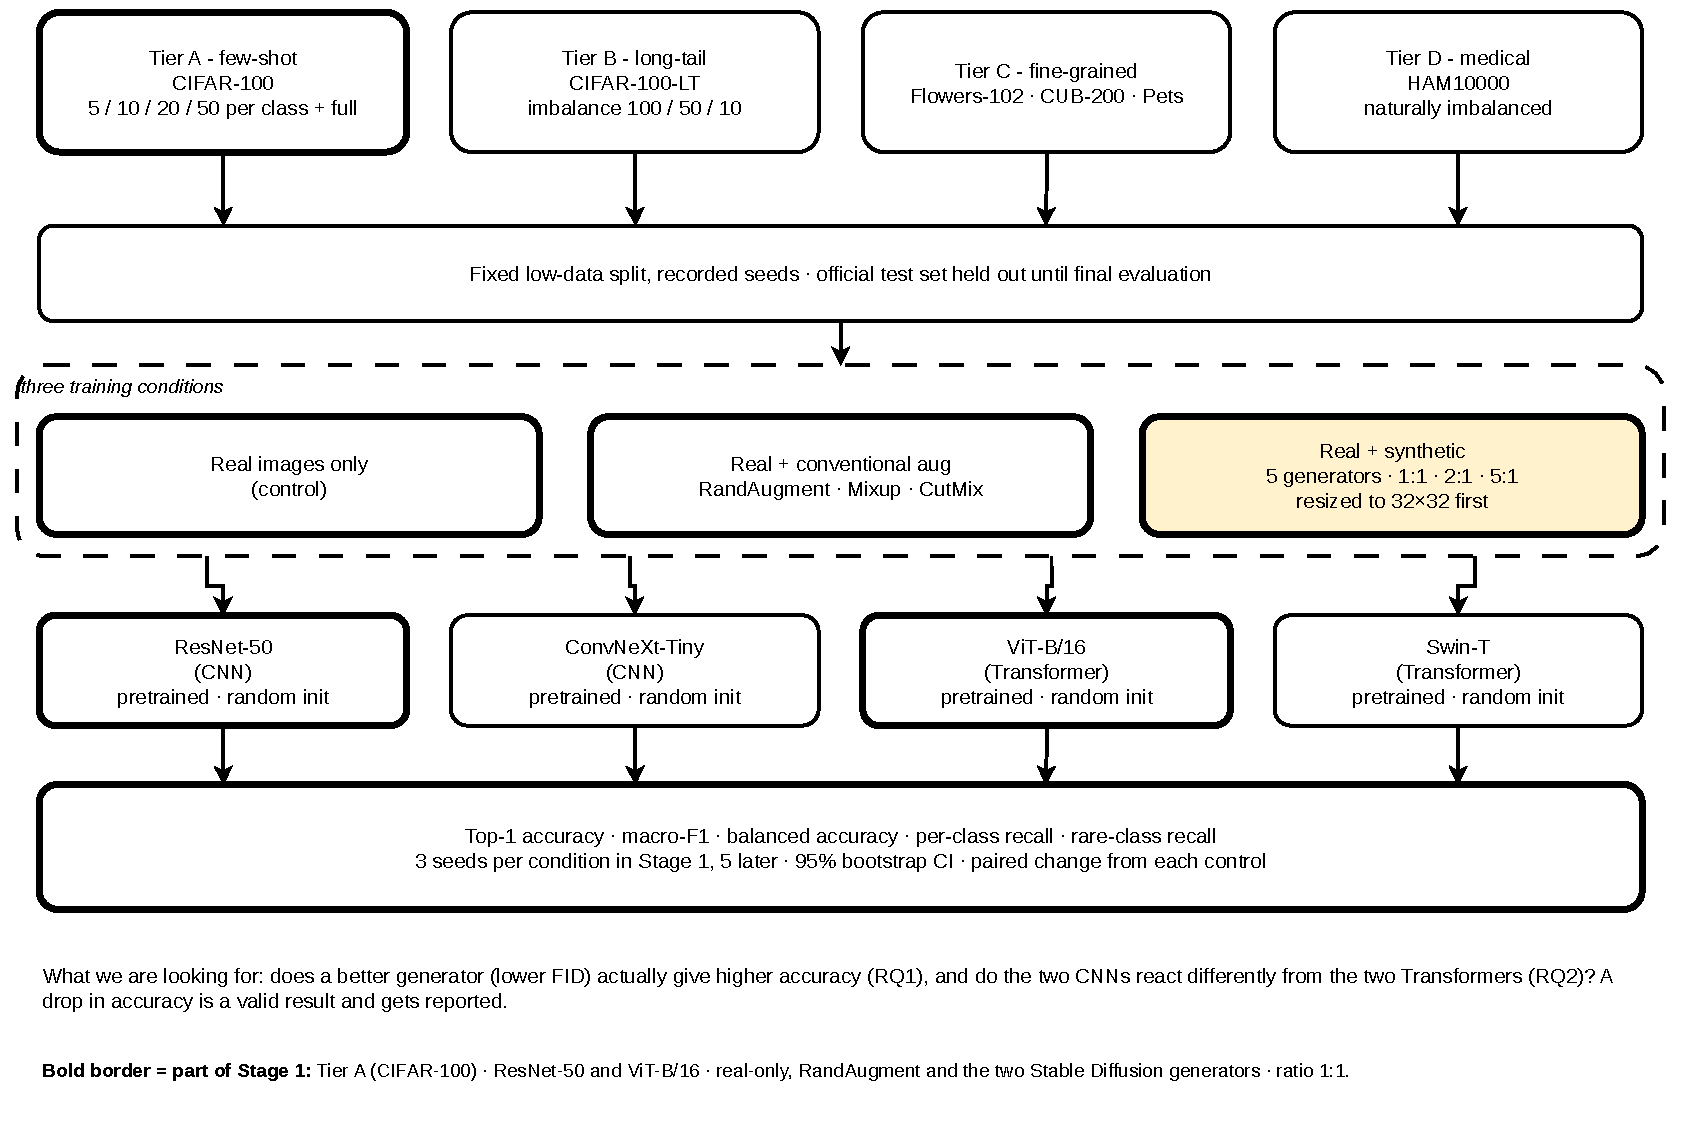
\includegraphics[width=\textwidth]{pipeline-2-classification.pdf}
	\caption{Classification study design. Each data tier is split once with recorded seeds, and the official
	test set is held out until the final evaluation. Every classifier, pretrained and randomly initialized,
	is trained under three conditions: real images only, real images with conventional augmentation, and
	real images with generated images, which are resized to the dataset's resolution first. Boxes with a
	bold border are part of Stage 1. \todo{redraw for the paper: only the CIFAR-100 tier and the
	classifiers and conditions that were run, plus the GAN set; drop the ``Stage 1'' wording}}
	\label{fig:classification-design}
\end{figure}
